\chapter{rComplexity in Practice}


\section{Human-driven calculus of rComplexity}
This section aims to present a simple methodology of calculating by hand the associated rComplexity class for any given algorithm, provided a predefined instruction set architecture and the correspondence between generic instructions and required time for execution as well as enhanced hardware designs details related to the total execution time (no. of stages of pipeline, scalability degree, etc.)\cite{hennessy2011computer}. Even if the process of calculating an exact rComplexity class associated to a real algorithm is unpractical, the method provided can be applied with colossal endeavor. Later on, we will present an automated method of estimating the rComplexity of a given algorithm.

\subsection{N-Queens’ Problem}


As a fundamental process-key in testing the capacity of the AI in solving various problems together with that of creating low-complexity algorithms, N queens counts as one of the most applicable and explored programmes in the field of mathematics and programming. Being initially designed as a solution of Max Bezzel’s 8 queens puzzle (proposed in 1848), that by Franz Nauck created the generalized puzzle for the known N-queens problem.

Due to movement complexity of queens, the increased number of required computations as the size of the input increases(time complexity grows fast), and the vast number of possible board states, N-queens problem has been explored by mathematicians and programmers quite extensively.

\begin{figure}[H]
    \centering
    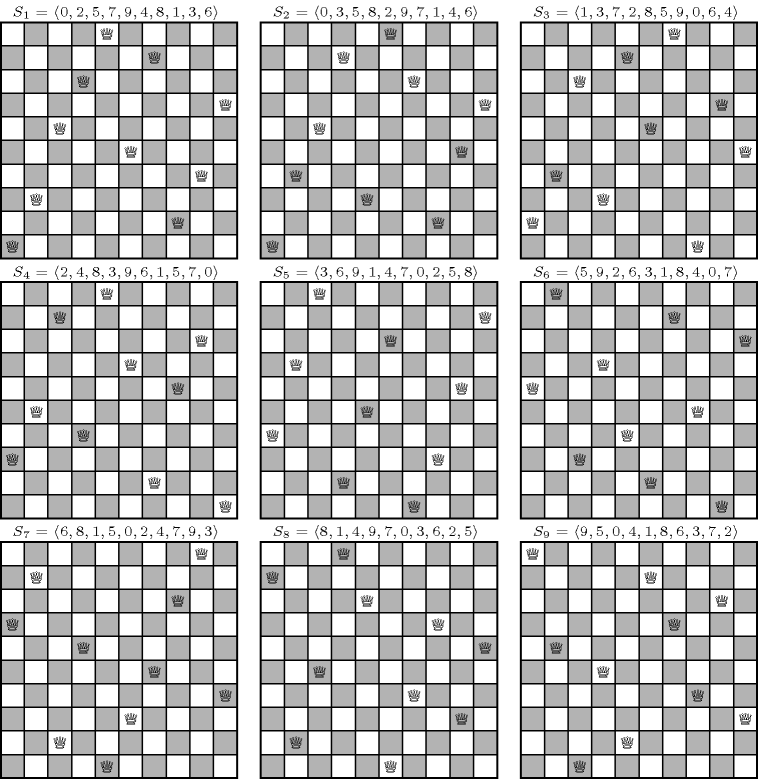
\includegraphics[width=0.5\textwidth]{nqueen_sol10}
    \caption{Possible solutions for $n=10$}
\end{figure}

This subsection proposes a naive solution. In order to begin to solve this problem,an observation about choosing the $N$ Queens on the board with the dimensions $n$ x $n$ is needed. In order not to have attacks between two Queens, it must not have two Queens on the same line or column.


We define a Queen $Q$ by the pair on points $ (x, y) $, where $ x, y \leq n $, are the coordinates corresponding to the position on the chessboard.

The problem can be solved by checking all possible permutations:

$ Q (1) = (1, y_1) $ , $ Q (2) = (2, y_2) $ ... , $ Q (n) = (n, y_n) $ \\
where $ y_1, y_2, ..., y_n \ in \ { 1,2, ..., n \ } $ and $ y_1, y_2, ..., y_n $ distinct.

In these conditions, the only action that still needs to be verified is that of the \textit{"diagonal attack"} of any two Queens.

\begin{algorithm}[H]
    \caption{Exhaustive N-Queens’ Problem Pseudocode}
    \begin{algorithmic}[1]
        \Procedure{QueenProblem}{$currentMatrix,row,column$}
        \If {$column=1$ and $row=n+1$}
        \State print currentMatrix
        \State Return

        \EndIf
        \For {i=1..n}
        \If {noConflict(currentMatrix,row,column) = TRUE}
        \State $currentMatrix[row][i] \gets 1$
        \State $QueenProblem(currentMatrix,row+1,1)$
        \State $currentMatrix[row][i] \gets 0$
        //BackTracking Step
        \EndIf
        \EndFor
        \EndProcedure
        \Procedure{Main}{$n$}


        \State $read\ n$
        \State $currentMatrix.initiate()$
        \State $currentMatrix.setrows(n)$
        \State $currentMatrix.setcolumns(n)$
        \State $currentMatrix \gets$
        $\left[\begin{array}{ccccc}
                   0 & 0 & ... & 0 & 0    \\
                   0 & 0 & ... & 0 & 0    \\
                   & & ... & &    \\
                   0 & 0 & ... & 0 & 0    \\
                   0 & 0 & ... & 0 & 0    \\
        \end{array}\right]$
        \State $QueenProblem(currentMatrix,1,1)$
        \EndProcedure
    \end{algorithmic}
\end{algorithm}

To begin with, a method of calculating traditional complexity using the classical model is presented hereby.
To calculate the complexity of the QueenProblem algorithm, we will individually analyze the complexities of the operations in the QueenProblem function. We will note with $n$ the number of Queens to be completed at a time $ t $ of the algorithm.

The matrix display operation occupies $ O (n ^ 2) $ (it represents a simple lookup in a $n\ x\ n$ matrix)

Each Queen Problem function calls other $ n $ instances, through recursive calls, of a smaller order with one unit complexity index ($ n-1 $).


\begin{algorithm}[H]
    \caption{noConflict Helper function}
    \begin{algorithmic}[1]
        \Procedure{noConflict}{$currentMatrix,row,column$}
        \For {i=1..row-1}
        \If {currentMatrix[i][column] = 1}
        \State \Return FALSE
        \EndIf
        \EndFor


        //Check on "diagonal" parallel with second diagonal
        \State $i \gets row$
        \For {j=column..n}
        \If {currentMatrix[i][j] = 1}
        \State \Return FALSE
        \EndIf
        \If {$i \leq 0$}
        \State break
        \EndIf
        \State $i \gets i-1$
        \EndFor

        //Check on "diagonal" parallel with main diagonal
        \State $i \gets row$
        \For {j=column..0 : increment -1}
        \If {currentMatrix[i][j] = 1}
        \State \Return FALSE
        \EndIf
        \If {$i \leq 0$}
        \State break
        \EndIf
        \State $i \gets i-1$
        \EndFor

        \EndProcedure

    \end{algorithmic}
\end{algorithm}

The forward and backtracking operations respectively are performed in $ O (1) $. The time consuming operation is the conflict checking operation (refer to the noConflict function defined below) that is performed in linear time $ O (n) $, because this function iterates, individually (only to the left of the created matrix), after the lines of the matrix (in $ O (n) $), after a diagonal parallel to the secondary diagonal of the matrix (in $ O (n) $) and after a diagonal parallel to the main diagonal of the matrix (in $ O (n) $).
Therefore:

$QueenProblem(n) = n \cdot QueenProblem(n-1) + n \cdot O(n),\ O(1)=O(n^2)$ \\
\noindent\rule{16cm}{0.4pt}
Proceeding to solving this equation:


$QueenProblem(n) = n \cdot QueenProblem(n-1) + n \cdot O(n) |\cdot\ 1$ \\
$QueenProblem(n-1) = (n-1) \cdot QueenProblem(n-2) + (n-1) \cdot O(n-1) |\cdot\ n-0$ \\
$QueenProblem(n-2) = (n-2) \cdot QueenProblem(n-3) + (n-2) \cdot O(n-2) |\cdot\ n\cdot (n-1)$ \\
$...$ \\
$QueenProblem(3) = 3 \cdot QueenProblem(2) + 3 \cdot O(3) |\cdot\ n\cdot (n-1) \cdot ... \cdot 3$ \\
$QueenProblem(2) = 2 \cdot QueenProblem(1) + 2 \cdot O(2) |\cdot\ n\cdot (n-1) \cdot ... \cdot 2$ \\
\noindent\rule{16cm}{0.4pt}
After computing the additions of the previously weighted equation, in a compact representation, the following result occurs:

\[QueenProblem(n) = n! \cdot QueenProblem(1) + \sum_{i=2}^{n} i\cdot O(i) \]
$QueenProblem(n) = n! \cdot O(n^2) + \sum_{i=2}^{n} O(i^2)$ \\
$QueenProblem(n) = n! \cdot O(n^2) + O(\sum_{i=2}^{n} i^2)$ \\
$QueenProblem(n) = n! \cdot O(n^2) + O(\dfrac{n\cdot(n+1)\cdot(2n+1)}{6} - 1)$ \\
$QueenProblem(n) = n! \cdot O(n^2) + O(n^3)$ \\
$QueenProblem(n) = O(n! \cdot n^2 + n^3) $ \\

Then, the Bachmann–Landau associated Big $O$-complexity class for the given algorithm is:
\[QueenProblem(n) = O(n^2\cdot n!) \]

\noindent\rule{16cm}{0.4pt}

rComplexity calculus is similar, but it requires higher precision of class approximation and additional architectural aspects.
First change is that the noConflict function has it's performance dependent on the architecture, as not all CPU operations takes the same amount of CPU cycles.


For instance, for an x86 CPU, the associated rComplexity class would be
$ O_{1}(c_{noConflict} * n) $, where $c_{noConflict}$ is a constant corresponding to the no. of cycles required to perform the operations inner the for-loop.

For the pseudocode:
\begin{algorithmic}[1]
    \For {i=1..row-1}
    \If {currentMatrix[i][column] = 1}
    \State \Return FALSE
    \EndIf
    \EndFor
\end{algorithmic}
In a broad manner, we can estimate that the cost for the inner snippet is $c_{computeOffset} + c_{readMemory} + c_{check=1}$, where in order to compute offset, we need to perform $i * ROWS + column$, so
$ c_{computeOffset} = O_{1}(c_{addition} + c_{multiplication} + 3 * c_{readMemory})$.


Seeking in a x86 Cycle cost table for various operations, we can estimate the primitives $c_{addition} = O_{1}(4)$ and $c_{multiplication} = O_{1}(4)$. For memory access, the time varies, on reasons based on cache mechanics, prefetch and other runtime mechanism for improvement in speed of read operations. A satisfying margin would be $c_{readMemory} = O_{1}(100)$.

\begin{figure}[H]
    \centering
    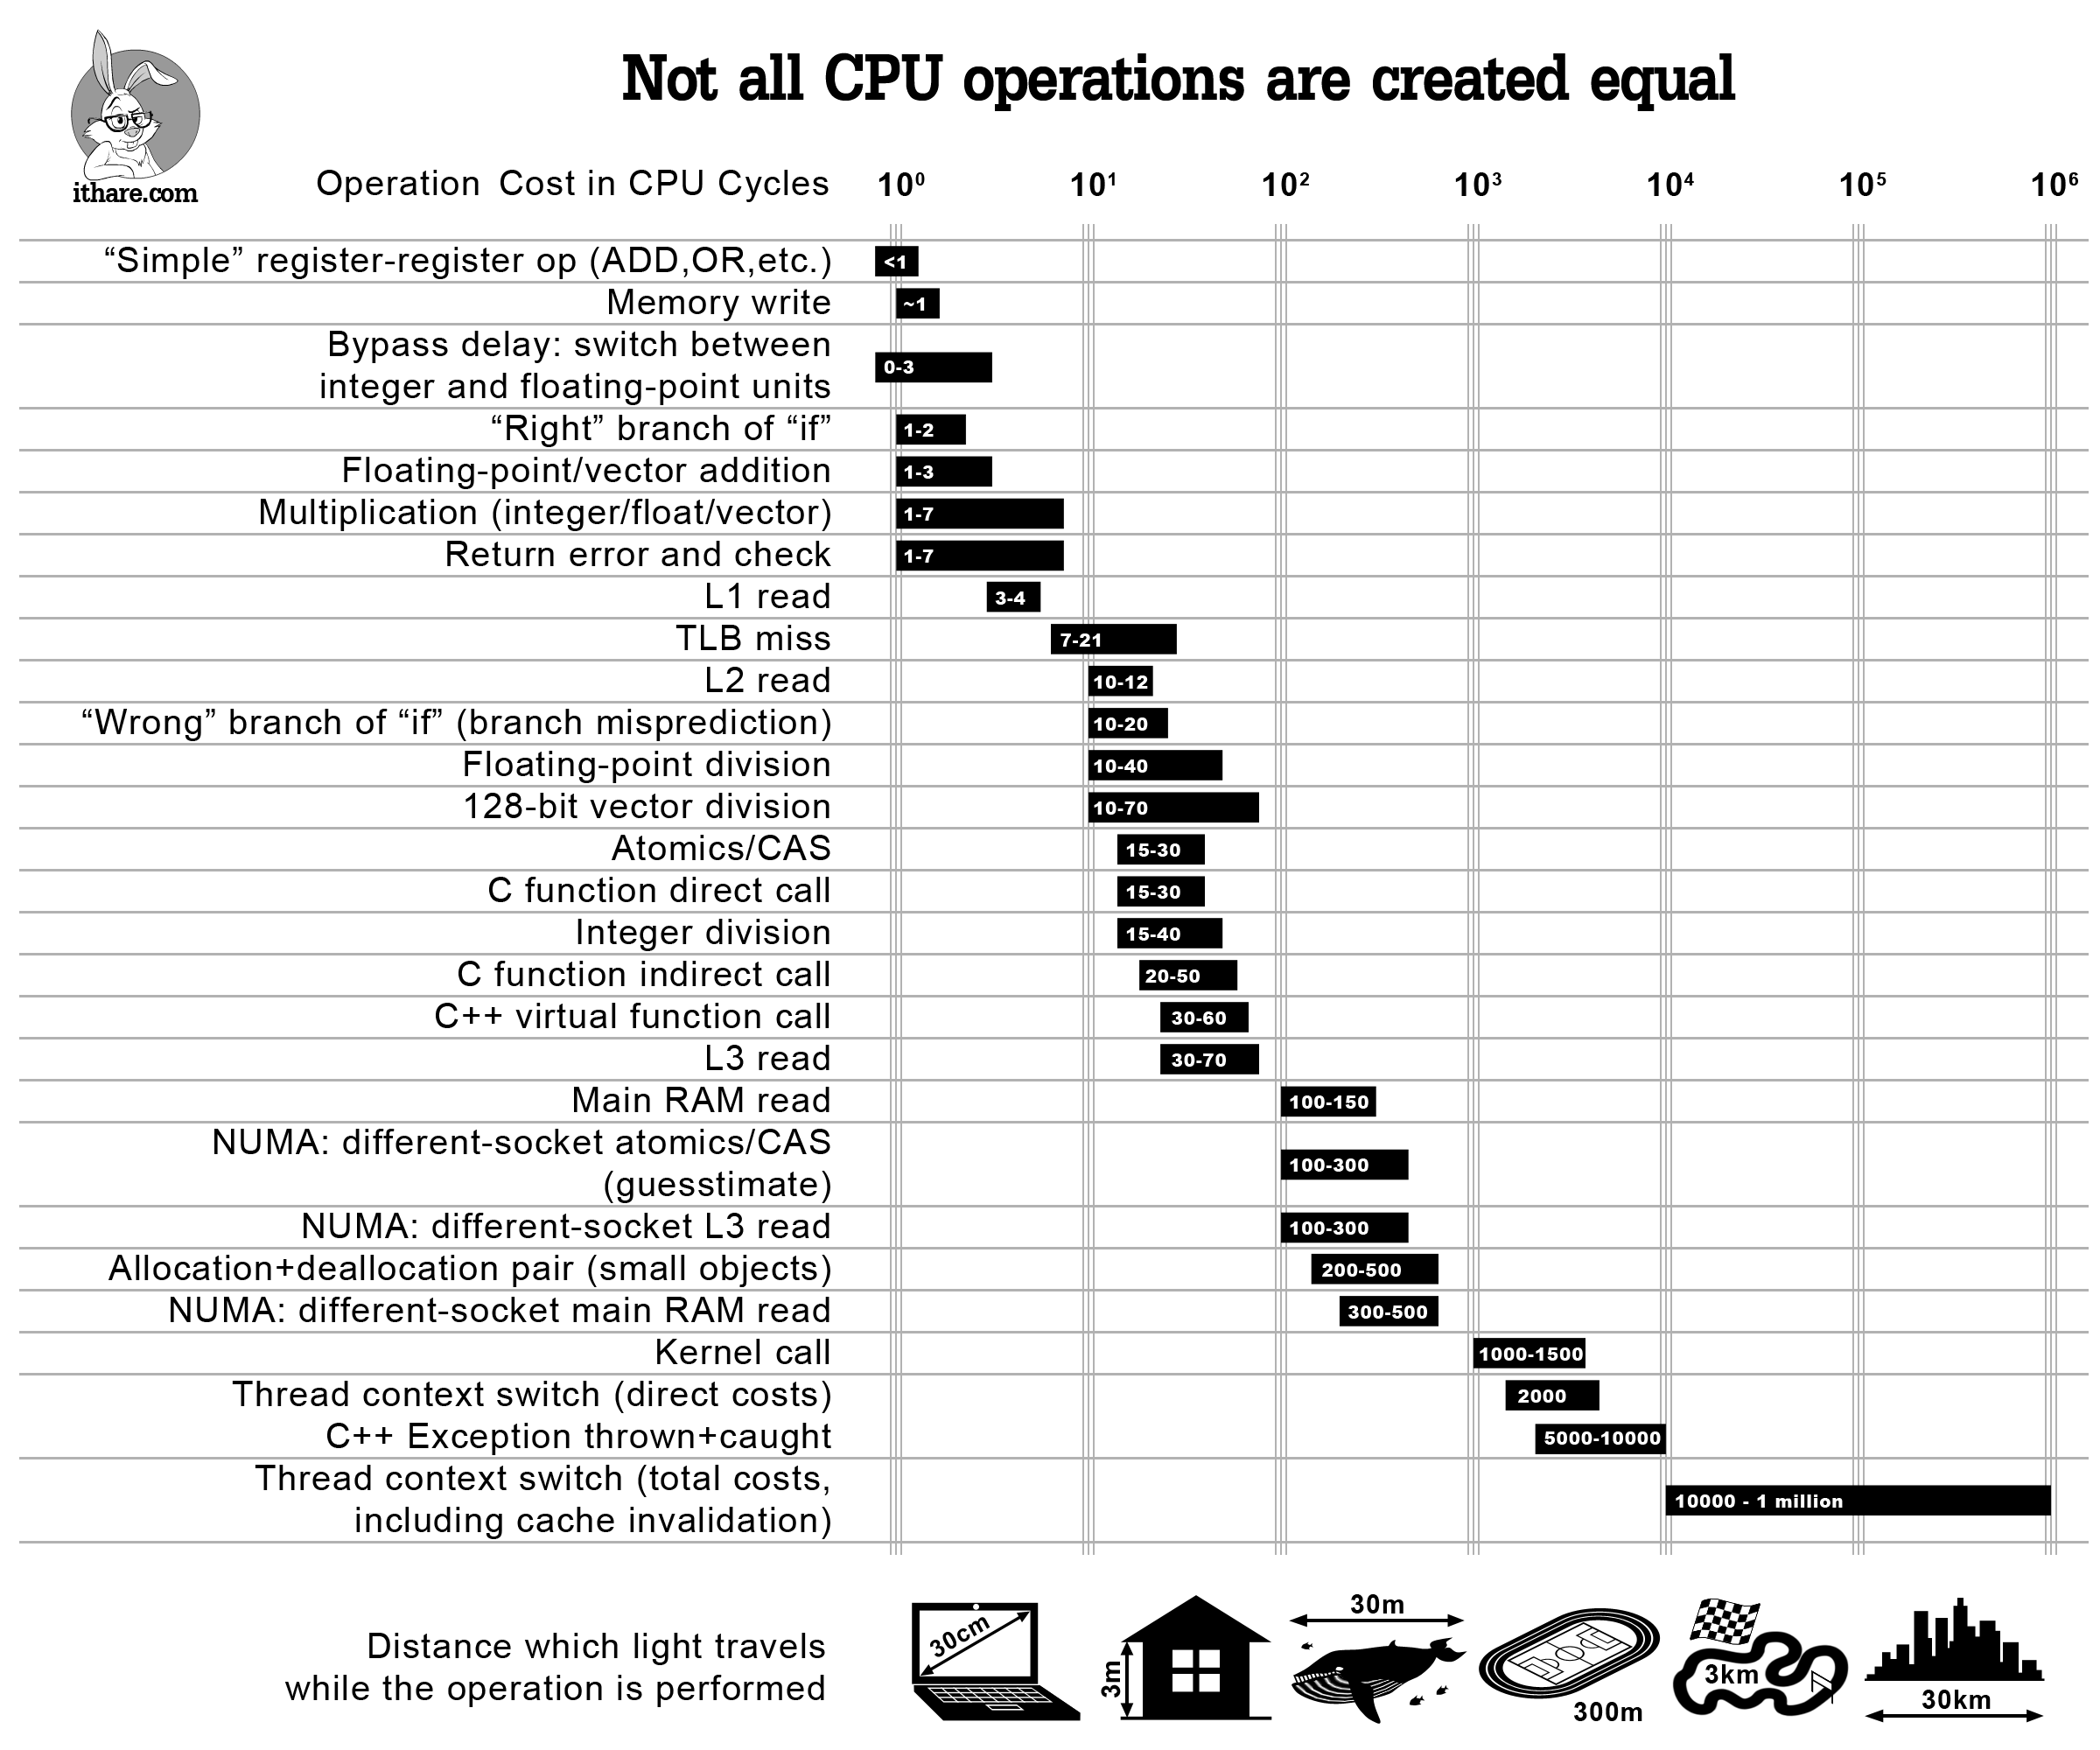
\includegraphics[width=0.95\textwidth]{part101_infographics_v08}
    \caption{Averages of the Costs (in CPU Clock Cycles) for the fundamental assembly instructions \cite{archcost}}
\end{figure}

Suppose for a complete check and jump at an pre-computed address $c_{check=1} = 10$.

Therefore, for the inner snippet using the above estimations, the rComplexity would be $O_{1}(4 * 100 + 4 + 4 + 10) = O_{1}(418)$. Now, the whole snippet will have the complexity $O_{1}((418 + c_{for\_checks}) \cdot n)$, where  $c_{for\_checks} = c_{check=row} + c_{addition}$ is the associated cost for incrementing the index and other checks.

Thus, the rComplexity of the snippet is $O_{1}((418 + 14) \cdot n) = O_{1}(432 \cdot n)$ using the above estimations.


For an exact value, we need to check the associated generated assembly code for the architecture (example x86-32bit):
\begin{verbatim}
f:
    push ebp
    mov ebp, esp
    sub esp, 16
    mov DWORD PTR [ebp-4], 0
    jmp .L2
.L5:
    mov eax, DWORD PTR [ebp-4]
    imul edx, eax, 400 # for a 20x20 board
    mov eax, DWORD PTR [ebp+16]
    add edx, eax
    mov eax, DWORD PTR [ebp+12]
    mov eax, DWORD PTR [edx+eax*4]
    cmp eax, 1
    je .L6
    add DWORD PTR [ebp-4], 1
.L2:
    mov eax, DWORD PTR [ebp-4]
    cmp eax, DWORD PTR [ebp+8]
    jl .L5
    jmp .L1
.L6:
    nop
.L1:
    leave
    ret
\end{verbatim}


The inner loop calculus are provided inner $.L5$ label. Having this code and the x86 cycles/instructions table, we can calculate the ideal rComplexity $\Theta_{1}(n \cdot (c_{.L2} + c_{.L5}))$.

Also, $c_{.L2} = c_{mov} + c_{cmp} + c_{li}$ and $c_{.L5} = c_{mov} + c_{imul} + c_{mov} + c_{add} + c_{mov} + c_{mov} + c_{cmp} + c_{je} + c_{add} $.

Using reflexivity, we conclude the rComplexity of the snippet 1 is \[f_{snippet_{1}} =  \Theta_{1}(n \cdot ( 5 * c_{mov} + c_{imul} + 2 * c_{add} +2 *  c_{cmp} + c_{je} + c_{li}))\]

Having this snippet's associated complexity calculated, we can proceed to calculate the other independent for-loops in the noConflict function:
\begin{algorithmic}[1]
    \For {j=column..n}
    \If {currentMatrix[i][j] = 1}
    \State \Return FALSE
    \EndIf
    \If {$i \leq 0$}
    \State break
    \EndIf
    \State $i \gets i-1$
    \EndFor
\end{algorithmic}
We will associate the complexity function of this snippet with $f_{snippet_{2}}$. Similarly, for the snippet:

\begin{algorithmic}[1]
    \For {j=column..0 : increment -1}
    \If {currentMatrix[i][j] = 1}
    \State \Return FALSE
    \EndIf
    \If {$i \leq 0$}
    \State break
    \EndIf
    \State $i \gets i-1$
    \EndFor
\end{algorithmic}
a complexity function will be obtained described by $f_{snippet_{3}}$.

Using addition properties, the complexity function for the procedute noConflict will be $f_{snippet_{1}} + f_{snippet_{2}} + f_{snippet_{3}} = O_{1}(c_{noConflict} \cdot n)$, where $c_{noConflict} \cdot n$ is the architecture-dependant constant.

For instance, for x86, we can approximate $c_{noConflict \cdot n} = 432 * 3 = 1296$ and $f_{snippet_{1}} + f_{snippet_{2}} + f_{snippet_{3}} = O_{1}(1296 \cdot n) $.


Going deeper, tracing the flow, we can evaluate the complexity of N-Queens Problem procedure by checking all elements involved in the procedure.
\[QueenProblem(n) = O_{1}(recursiveCall) + O_{1}(noConflict) + O_{1}(overhead) + O_{1}(basecase) \]
Therefore:
\[\begin{cases}
      QueenProblem(n) = n \cdot QueenProblem(n-1) + O_{1}(1296 \cdot n) (c_{overheadFor} + c_{setBitsMatrix}) \cdot O_{1}(n) \\ QueenProblem_{1}(1)=O_{1}(c_{printMatrix})
\end{cases}\]
where $O_{1}(1296 \cdot n)$ is the rComplexity for the noConflict check.

Using the previous estimation, we assume $c_{overheadFor} = 14$ and $c_{setBitsMatrix} = 108$. Thus, the recurrent equation looks as follows:
\[QueenProblem(n) = n \cdot QueenProblem(n-1) + O_{1}(1418 \cdot n) \]

For the base case, we need to compute the rComplexity of the $printMatrix$ method.
\[ \begin{cases}
       QueenProblem(1)=O_{1}(n^{2} \cdot  (c_{computeOffset} + c_{readMatrixElement})) \\ QueenProblem(1)=O_{1}(n^{2} \cdot  408)
\end{cases}\]

For simplicity, we can rewrite:
\[ \begin{cases}
       QueenProblem(n) = n \cdot QueenProblem(n-1) + 1418 \cdot O_{1}(n) \\ QueenProblem(1)= 408 \cdot O_{1}(n^{2})
\end{cases}\]

We can model the system as an recurrence equation:
\[ g(n) = n \cdot  g(n-1) + 1418 \cdot  n; g(0) = 408 \cdot  n^{2} \]
with the solution:
\[ 408 \cdot n^{3} \cdot \Gamma(n) + 1418 \cdot e \cdot  n \cdot \Gamma(n, 1)\]
where $\Gamma$ represents the \textit{gamma function} that satisfies: \[ \Gamma \left( x \right) = \int\limits_0^\infty {s^{x - 1} e^{ - s} ds} \] and $ \Gamma(n,x)$ represents the \textit{incomplete gamma function} that satisfies: \[ \Gamma \left(x, n \right) = \int\limits_n^\infty {s^{x - 1} e^{ - s} ds}\]

The solution of this recurrence equation in rComplexity calculus (with $n \in \mathbb{N}$) is:
\[ QueenProblem(n) = O_{1}(408 \cdot n^{2} \cdot n!) + O_{1}(1418 \cdot n \cdot n!) \]
Using the $O_{1}$ addition properties, we conclude:
\[ QueenProblem(n) = O_{1}(408 \cdot n^{2} \cdot n!) \]

\begin{remark}
    The rComplexity function associated with the algorithm $(408 \cdot n^{2} \cdot n!)$ is from the same tradition complexity class as calculated before $ O(n^2\cdot n!)$.
\end{remark}


\section{Automatic estimation of rComplexity}
This section aims to present a solution for automation for calculating an approximate of the associated rComplexity class for any given algorithm. The prerequisites for this method implies a technique for obtaining relevant metric-specific details for diversified input dimensions. For instance, if time is the monitored metric, there must exist a collection of pertinent data linking the correspondence between input size and the total execution time for the designated input size.

\subsection{Estimation for algorithms with known Bachmann–Landau Complexity}
Reckoning an associated rComplexity class ($f$) for an algorithm with established Bachmann–Landau Complexity ($g$) consists in the process of tailoring an suitable constant $c$, such that $f \approx \Theta_{1}(c \cdot g)$ or in Big-O calculus, $f \leq  \mathbb{O}_{1} (c \cdot g)$. The approach presented below is a particularized version of linear regression, which attempts to model the relationship between various variables by fitting a linear equation to observed data. Even if the model generally follows the classical pattern of a Machine Learning Process (training, predicting, etc.), where a training example consists of a pair ($inputSize$, $metricValue$).

A trick (frequently used in data science) is used to adjust the entry values if the Bachmann–Landau relationship between the $inputSize$ and the metric is known. In order to adjust the learning set to a more knowledgeable set, we can extract new features and replace all the ($inputSize$, $metricValue$) pairs with ($g(inputSize)$, $metricValue$), where $g$ is the known Bachmann–Landau Complexity function converted into Normal form.


The importance of this trick can be emphasized comparing the classical linear regression model with various learning datasets. For the matrix multiplication problem, a naive algorithm (with Bachmann–Landau Complexity $\mathbb{O}(n^{3})$) has been implemented. After testing, the algorithm has been deployed and executed matrix multiplications for various sizes of the matrixes. The execution has been audited and the results have been summarized in the following table, which represents the correspondance between matrix dimension and running time:

\begin{table}[H]
    \begin{center}
        \scalebox{0.5}{
            \begin{tabular}{|l|l|l|l|l|l|l|l|l|l|l|l|}
                \hline
                \begin{tabular}[c]{@{}l@{}}
                    input\\ Size
                \end{tabular} & Time $(s)$     & \begin{tabular}[c]{@{}l@{}}
                                                     input\\ Size
                \end{tabular} & Time $(s)$  & \begin{tabular}[c]{@{}l@{}}
                                                  input\\ Size
                \end{tabular} & Time $(s)$  & \begin{tabular}[c]{@{}l@{}}
                                                  input\\ Size
                \end{tabular} & Time $(s)$  & \begin{tabular}[c]{@{}l@{}}
                                                  input\\ Size
                \end{tabular} & Time $(s)$   & \begin{tabular}[c]{@{}l@{}}
                                                   input\\ Size
                \end{tabular} & Time $(s)$   \\ \hline
                16 & 0.000018 & 1024 & 8.52 & 2112 & 123.73 & 3200 & 462.71 & 4288 & 999.25 & 5376 & 1647.23 \\ \hline
                32 & 0.000339 & 1088 & 10.96 & 2176 & 135.21 & 3264 & 358.01 & 4352 & 864.15 & 5440 & 1929.46 \\ \hline
                48 & 0.001123 & 1152 & 13.76 & 2240 & 149.43 & 3328 & 540.64 & 4416 & 987.71 & 5504 & 1693.75 \\ \hline
                64 & 0.001468 & 1216 & 18.03 & 2304 & 148.82 & 3392 & 446.29 & 4480 & 1095.01 & 5568 & 1986.99 \\ \hline
                128 & 0.015482 & 1280 & 21.55 & 2368 & 180.07 & 3456 & 592.91 & 4544 & 1126.39 & 5632 & 2002.14 \\ \hline
                256 & 0.084991 & 1344 & 25.59 & 2432 & 117.83 & 3520 & 480.98 & 4608 & 1147.28 & 5696 & 2013.22 \\ \hline
                320 & 0.172411 & 1408 & 30.66 & 2496 & 213.51 & 3584 & 621.36 & 4672 & 1280.23 & 5760 & 2066.87 \\ \hline
                384 & 0.296398 & 1472 & 28.27 & 2560 & 236.41 & 3648 & 582.46 & 4736 & 1228.73 & 5824 & 2029.52 \\ \hline
                448 & 0.535461 & 1536 & 41.91 & 2624 & 255.39 & 3712 & 628.36 & 4800 & 1222.14 & 5888 & 2236.73 \\ \hline
                512 & 0.764842 & 1600 & 48.90 & 2688 & 275.05 & 3776 & 650.76 & 4864 & 1256.73 & 5952 & 2503.13 \\ \hline
                576 & 1.308485 & 1664 & 56.34 & 2752 & 167.51 & 3840 & 651.43 & 4928 & 1290.35 & 6016 & 2317.91 \\ \hline
                640 & 1.803608 & 1728 & 70.47 & 2816 & 268.64 & 3904 & 626.79 & 4992 & 1488.43 & 6080 & 2395.12 \\ \hline
                704 & 2.516613 & 1792 & 71.02 & 2880 & 296.00 & 3968 & 659.29 & 5056 & 1432.41 & 6144 & 2718.02 \\ \hline
                768 & 3.334002 & 1856 & 84.41 & 2944 & 304.91 & 4032 & 915.86 & 5120 & 1093.62 & &         \\ \hline
                832 & 4.315076 & 1920 & 67.05 & 3008 & 300.06 & 4096 & 769.01 & 5184 & 1649.00 & &         \\ \hline
                896 & 5.571474 & 1984 & 99.74 & 3072 & 228.34 & 4160 & 864.89 & 5248 & 1729.42 & &         \\ \hline
                960 & 7.076612 & 2048 & 110.90 & 3136 & 446.72 & 4224 & 789.13 & 5312 & 1743.26 & &         \\ \hline
            \end{tabular}
        }
    \end{center}
    \caption{Reported timings for different input size for a naive matrix multiplication algorithm in $\mathbb{O}(n^{3})$. Results have been obtained on an i5 3.2GHz, x86\_64 Architecture with L1d cache: 32K, L1i cache: 32K, L2 cache: 256K, L3 cache: 6144K}
\end{table}

Training a linear regression model on this dataset would result in model with a linear equation to observed data, similar with the one below(a). Changes in the original dataset can enhance fitting results for the regression.

Examples for ($inputSize$, $metricValue$) $ \Rightarrow $ ($inputSize^{n}$, $metricValue$) are presented in (b) $n = 2$, (c) $n = 3$ and (d) $n = 4$.


\begin{table}[H]
    \begin{center}
        \scalebox{0.5}{
            \begin{tabular}{|l|l|l|l|l|l|l|l|l|l|l|l|}
                \hline
                \begin{tabular}[c]{@{}l@{}}
                    input\\ Size$^3$
                \end{tabular} & Time $(s)$     & \begin{tabular}[c]{@{}l@{}}
                                                     input\\ Size$^3$
                \end{tabular} & Time $(s)$  & \begin{tabular}[c]{@{}l@{}}
                                                  input\\ Size$^3$
                \end{tabular} & Time $(s)$  & \begin{tabular}[c]{@{}l@{}}
                                                  input\\ Size$^3$
                \end{tabular} & Time $(s)$  & \begin{tabular}[c]{@{}l@{}}
                                                  input\\ Size$^3$
                \end{tabular} & Time $(s)$   & \begin{tabular}[c]{@{}l@{}}
                                                   input\\ Size$^3$
                \end{tabular} & Time $(s)$   \\ \hline
                4.10E+03 & 0.000018 & 1.07E+09 & 8.52 & 9.42E+09 & 123.73 & 3.28E+10 & 462.71 & 7.88E+10 & 999.25 & 1.55E+11 & 1647.23 \\ \hline
                3.28E+04 & 0.000339 & 1.29E+09 & 10.96 & 1.03E+10 & 135.21 & 3.48E+10 & 358.01 & 8.24E+10 & 864.15 & 1.61E+11 & 1929.46 \\ \hline
                1.11E+05 & 0.001123 & 1.53E+09 & 13.76 & 1.12E+10 & 149.43 & 3.69E+10 & 540.64 & 8.61E+10 & 987.71 & 1.67E+11 & 1693.75 \\ \hline
                2.62E+05 & 0.001468 & 1.80E+09 & 18.03 & 1.22E+10 & 148.82 & 3.90E+10 & 446.29 & 8.99E+10 & 1095.01 & 1.73E+11 & 1986.99 \\ \hline
                2.10E+06 & 0.015482 & 2.10E+09 & 21.55 & 1.33E+10 & 180.07 & 4.13E+10 & 592.91 & 9.38E+10 & 1126.39 & 1.79E+11 & 2002.14 \\ \hline
                1.68E+07 & 0.084991 & 2.43E+09 & 25.59 & 1.44E+10 & 117.83 & 4.36E+10 & 480.98 & 9.78E+10 & 1147.28 & 1.85E+11 & 2013.22 \\ \hline
                3.28E+07 & 0.172411 & 2.79E+09 & 30.66 & 1.56E+10 & 213.51 & 4.60E+10 & 621.36 & 1.02E+11 & 1280.23 & 1.91E+11 & 2066.87 \\ \hline
                5.66E+07 & 0.296398 & 3.19E+09 & 28.27 & 1.68E+10 & 236.41 & 4.85E+10 & 582.46 & 1.06E+11 & 1228.73 & 1.98E+11 & 2029.52 \\ \hline
                8.99E+07 & 0.535461 & 3.62E+09 & 41.91 & 1.81E+10 & 255.39 & 5.11E+10 & 628.36 & 1.11E+11 & 1222.14 & 2.04E+11 & 2236.73 \\ \hline
                1.34E+08 & 0.764842 & 4.10E+09 & 48.90 & 1.94E+10 & 275.05 & 5.38E+10 & 650.76 & 1.15E+11 & 1256.73 & 2.11E+11 & 2503.13 \\ \hline
                1.91E+08 & 1.308485 & 4.61E+09 & 56.34 & 2.08E+10 & 167.51 & 5.66E+10 & 651.43 & 1.20E+11 & 1290.35 & 2.18E+11 & 2317.91 \\ \hline
                2.62E+08 & 1.803608 & 5.16E+09 & 70.47 & 2.23E+10 & 268.64 & 5.95E+10 & 626.79 & 1.24E+11 & 1488.43 & 2.25E+11 & 2395.12 \\ \hline
                3.49E+08 & 2.516613 & 5.75E+09 & 71.02 & 2.39E+10 & 296.00 & 6.25E+10 & 659.29 & 1.29E+11 & 1432.41 & 2.32E+11 & 2718.02 \\ \hline
                4.53E+08 & 3.334002 & 6.39E+09 & 84.41 & 2.55E+10 & 304.91 & 6.55E+10 & 915.86 & 1.34E+11 & 1093.62 & &         \\ \hline
                5.76E+08 & 4.315076 & 7.08E+09 & 67.05 & 2.72E+10 & 300.06 & 6.87E+10 & 769.01 & 1.39E+11 & 1649.00 & &         \\ \hline
                7.19E+08 & 5.571474 & 7.81E+09 & 99.74 & 2.90E+10 & 228.34 & 7.20E+10 & 864.89 & 1.45E+11 & 1729.42 & &         \\ \hline
                8.85E+08 & 7.076612 & 8.59E+09 & 110.90 & 3.08E+10 & 446.72 & 7.54E+10 & 789.13 & 1.50E+11 & 1743.26 & &         \\ \hline
            \end{tabular}
        }
    \end{center}
    \caption{Training data for the linear regression model after mapping ($inputSize$, $metricValue$) pairs with ($inputSize^3$, $metricValue$)}
\end{table}


As an intuition (due to the associated complexity function $O(n^3)$ in the Bachmann–Landau Complexity model), the natural fit was obtained when using $g(n) = n^3$ with consideration to generalization. If we choose much much bigger degree polynomial transformations, we may obtain better results on this datasets, but the models are becoming subject to overfit.

The subject of Matrix multiplication is furthered discussed in a distinct section.

\begin{figure}[H]
    \makebox[\textwidth][c]{\parbox{1.2\textwidth}{%
        \begin{subfigure}{.6\textwidth}
            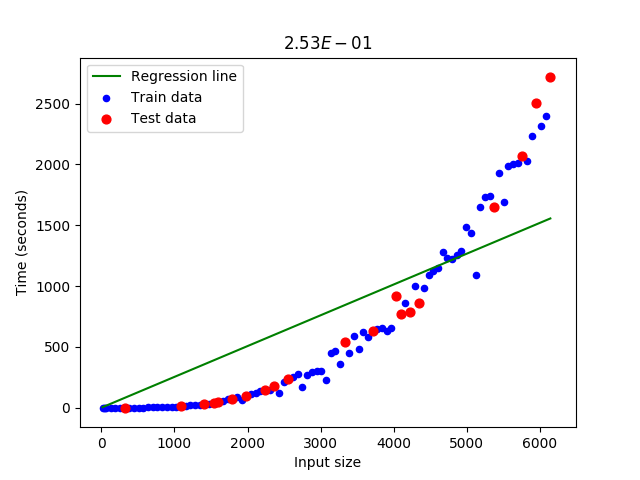
\includegraphics[width=\linewidth]{mm521_1.png}
            \caption{Linear Regression Model trained with features \\ obtained using the transformation $g(n) = n^1 $}
        \end{subfigure}%
        \begin{subfigure}{.6\textwidth}
            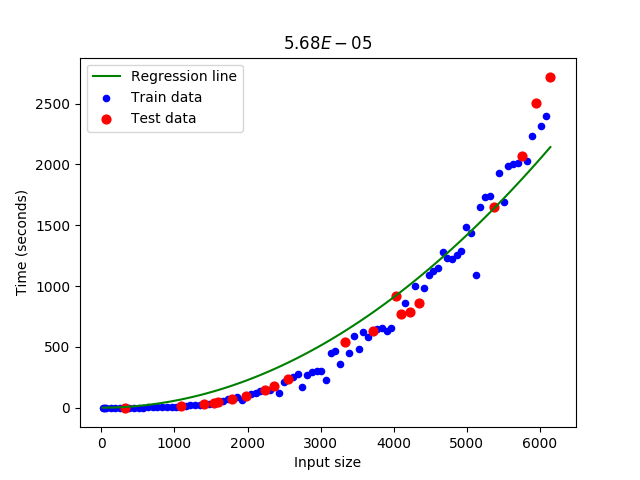
\includegraphics[width=\linewidth]{mm521_2.png}
            \caption{Linear Regression Model trained with features \\ obtained using the transformation $g(n) = n^2 $}
        \end{subfigure}
        \begin{subfigure}{.6\textwidth}
            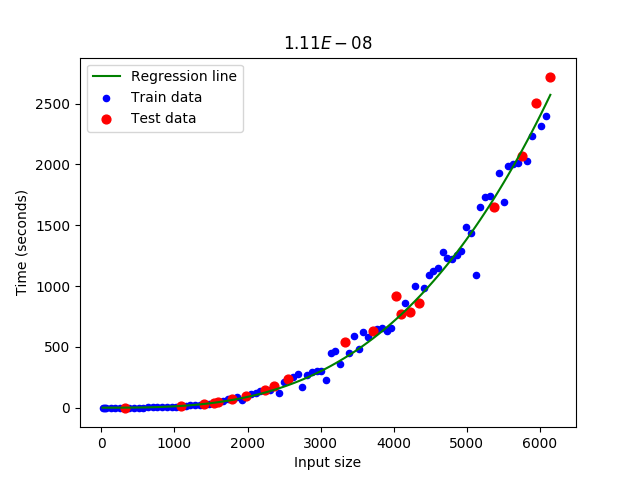
\includegraphics[width=\linewidth]{mm521_3.png}
            \caption{Linear Regression Model trained with features \\ obtained using the transformation $g(n) = n^3$}
        \end{subfigure}%
        \begin{subfigure}{.6\textwidth}
            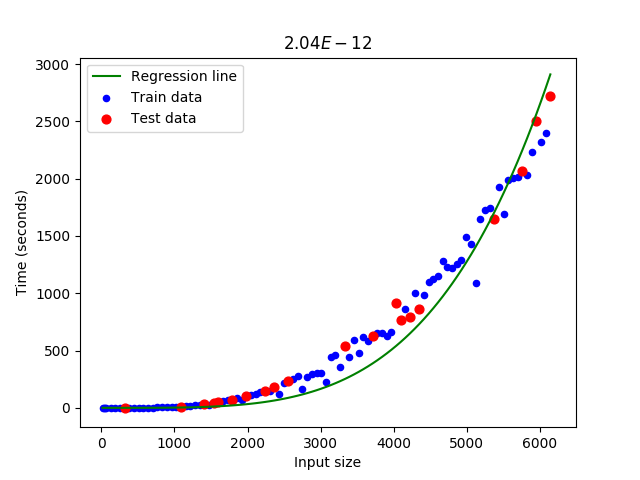
\includegraphics[width=\linewidth]{mm521_4.png}
            \caption{Linear Regression Model trained with features \\ obtained using the transformation $g(n) = n^4$}
        \end{subfigure}
    }}
    \caption{Various prediction boundaries based on accommodated training dataset using multiple relations $g$. Training data are obtained for different input size for a naive matrix multiplication algorithm in $\mathbb{O}(n^{3})$}
\end{figure}

\subsection{Estimation for algorithms with unknown Bachmann–Landau Complexity}
Estimation for algorithms with unknown Bachmann–Landau Complexity becomes a lot more difficult as there are numerous possible candidates for a matching complexity function.

A general polynomial Performance model normal form is presented in Chapter 2.1 Automatic Empirical Performance Modeling of Parallel Programs \cite{calotoiu2018automatic}. An enhance model for complexity functions should contain also an exponential behavior, which is often seen as a synergy between NP-Hard problems. Thus, we propose the following general expression:

\[ f(n) =\sum\limits_{t=1}^{y}  \sum\limits_{k=1}^{x} c_{k} \cdot n^{p_{k}} \cdot log_{l_{k}}^{j_{k}}(n) \cdot e_{t}^{n} \cdot  \Gamma(n)^{g_{k}} \]
This representation is, of course, not exhaustive, but it works in most practical schemes. An intuitive motivation is a consequence of how most computer algorithms are designed. \cite{calotoiu2018automatic}


\section{Matrix multiplication}
In this section, we aim to provide an example of estimation for matrix multiplication algorithms with known Bachmann–Landau Complexity.

Matrix multiplication plays very important role in many scientific disciplines because of fact that it is considered as the main tool for many other computations in different areas, like those in seismic analysis, different simulations (like galactic simulations), aerodynamic computations, signal and images processing. \cite{4588528}


\begin{figure}[H]
    \centering
    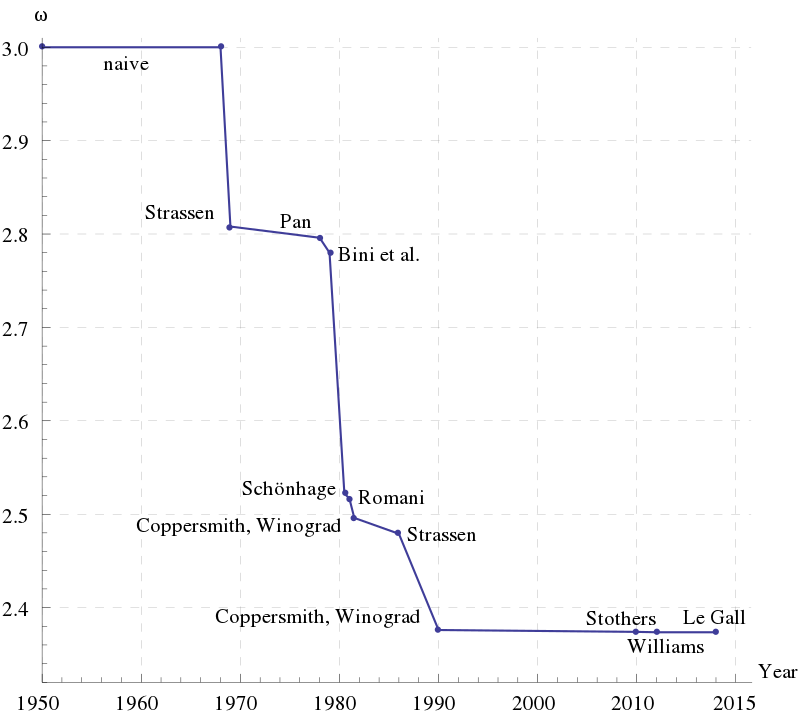
\includegraphics[width=0.4\textwidth]{matrixC}
    \caption{Before 1969, all known matrix multiplication algorithm were in $O(n^3)$. After Volker Strassen first published this algorithm and proved that the naive algorithm wasn't optimal, various attempts to narrow down the exponent $\omega$ appeared. One big breakthrough was brought by Coppersmith–Winograd algorithm, with complexity $O(n^{2.375})$. }
\end{figure}

\subsection{Naive and optimized implementations}
We analyzed various naive matrix multiplication algorithms $O(n^3)$ with memory-access improvements (cache-locality of loops, Blocked Matrix Multiplication) and an efficient implementation of Strassen algorithm.

\begin{figure}[H]
    \centering
    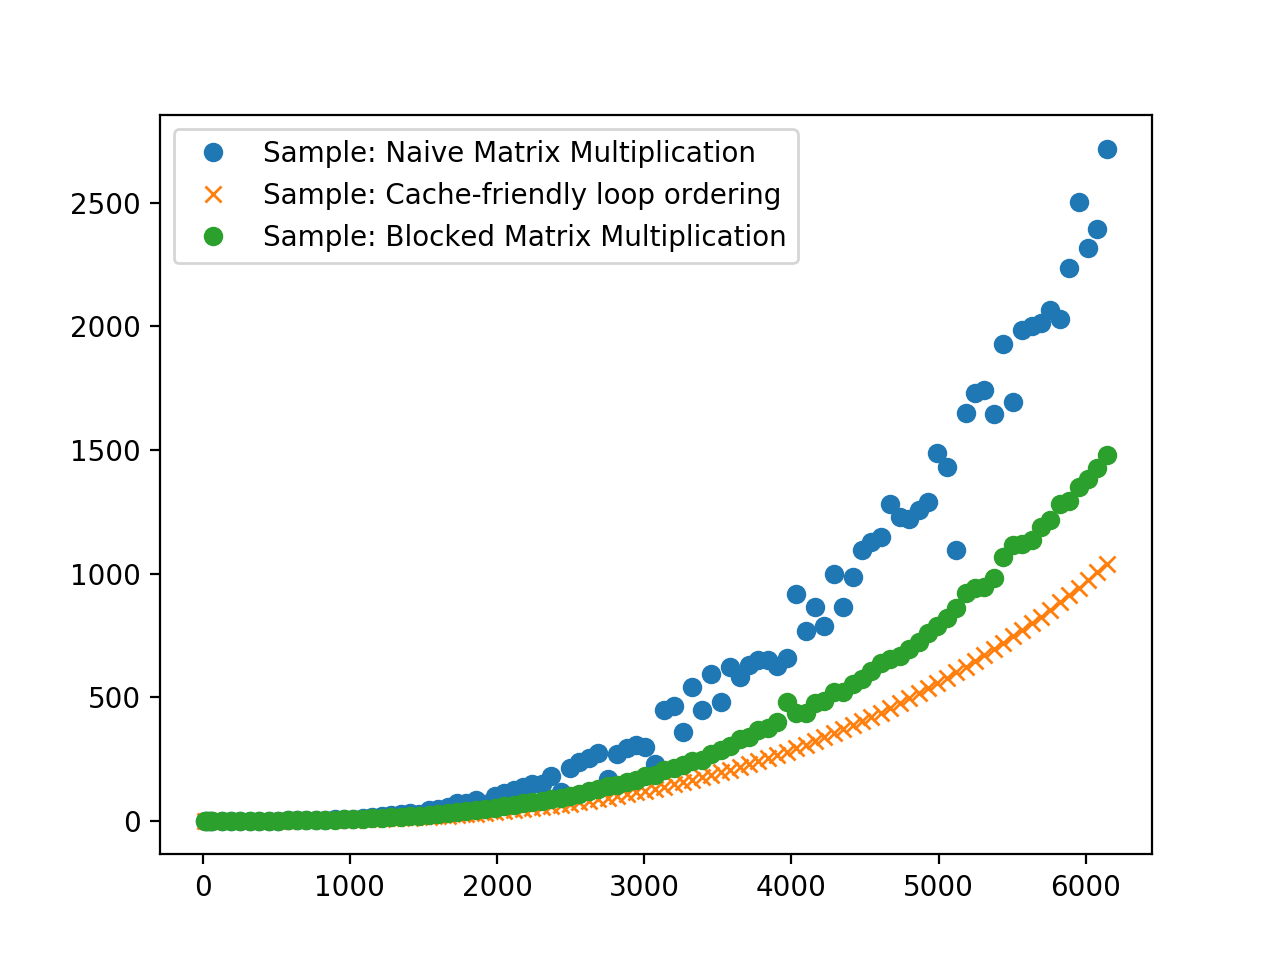
\includegraphics[width=0.7\textwidth]{matrixn3all}
    \caption{The results above have been reported on an i5 3.2GHz, x86\_64 Architecture with L1d cache: 32K, L1i cache: 32K, L2 cache: 256K, L3 cache: 6144K. We do not postulate that the methods above cannot be enhanced
    or the efficiency of the optimizations are in a specific order. We aim to provide various estimation for these implementations of matrix multiplication algorithms with known $O(n^3)$ Complexity. Please remark the natural distribution of the two cache-friendly algorithms presented on larger datasets vs the naive algorithm, susceptible to outliers.}
\end{figure}

Using the method described in estimating section, we can tailor an architecture-specific complexity function $ f(n)  = c \cdot n^3$.

\begin{figure}[H]
    \centering
    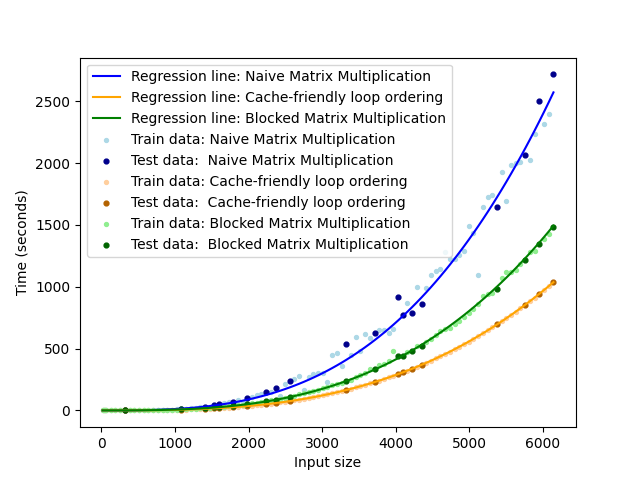
\includegraphics[width=0.7\textwidth]{mmn3023}
    \caption{Regression lines corresponding to each of the matrix-multiplication algorithms}
\end{figure}

After training the regression models for each algorithm, we obtained the coefficients $c$, that defines the complexity function $f(n)  = c \cdot n^3$.
\begin{table}[H]
    \centering
    \begin{tabular}{|
    >{\columncolor[HTML]{FFCCC9}}l |
    >{\columncolor[HTML]{32CB00}}l |}
        \hline
        \cellcolor[HTML]{C0C0C0}\textit{\textbf{Algorithm}} & \cellcolor[HTML]{C0C0C0}{\color[HTML]{000000} \textit{\textbf{\begin{tabular}[c]{@{}l@{}}
                                                                                                                                Complexity Function
        \end{tabular}}}} \\ \hline
        \textbf{Naive Matrix Multiplication}                & {$ O_{1}(1.109 \cdot 10^{-8} \cdot n^3 \cdot HZ) $}                                                                                      \\ \hline
        \textbf{Cache-friendly loop ordering}               & {$ O_{1}(4.472 \cdot 10^{-9} \cdot n^3 \cdot HZ) $ }                                                                                      \\ \hline
        \textbf{Blocked Matrix Multiplication}              & {$ O_{1}(6.441 \cdot 10^{-9} \cdot n^3 \cdot HZ) $ }                                                                                      \\ \hline
    \end{tabular}
    \caption{In this representation, the complexity function is scaled to produce output in seconds. In order to obtain rComplexity function, multiplying with processor frequency is mandatory $HZ \approx 3.2 \cdot 10^9 $. The regression model was evaluating using the above metrics: Root Mean Square Error (RMSE) and $R^2$ (coefficient of determination) regression score function}
\end{table}


Furthermore, the model was evaluated adopting classical regression evaluation metrics, independently settled on training and testing data.
\begin{table}[H]
    \begin{tabular}{|
    >{\columncolor[HTML]{FFCCC9}}l |
    >{\columncolor[HTML]{32CB00}}l |
    >{\columncolor[HTML]{FFFFFF}}l |
    >{\columncolor[HTML]{FFFFFF}}l |
    >{\columncolor[HTML]{FFFFFF}}l |
    >{\columncolor[HTML]{FFFFFF}}l |}
        \hline
        \cellcolor[HTML]{C0C0C0}\textit{\textbf{Algorithm}} & \cellcolor[HTML]{C0C0C0}{\color[HTML]{000000} \textit{\textbf{c}}} & \cellcolor[HTML]{C0C0C0}\textit{\begin{tabular}[c]{@{}l@{}}{[}
                                                                                                                                                                       Training{]}\\ RMSQ\end{tabular}} & \cellcolor[HTML]{C0C0C0}\textit{\begin{tabular}[c]{@{}l@{}}{[}Training{]}\\ R2 score\end{tabular}} & \cellcolor[HTML]{C0C0C0}\begin{tabular}[c]{@{}l@{}}{[}Test{]}\\ RMSQ:\end{tabular} & \cellcolor[HTML]{C0C0C0}\textit{\begin{tabular}[c]{@{}l@{}}{[}Test{]}\\ R2 score\end{tabular}} \\ \hline
\textbf{Naive Matrix Multiplication}                & {\color[HTML]{000000} \textit{1.109e-08}}                          & {\color[HTML]{000000} 5740.95}                                                                     & 0.9886 & 6136.10 & {\color[HTML]{000000} 0.9912}                                                                      \\ \hline
\textbf{Cache-friendly loop ordering}               & {\color[HTML]{000000} \textit{4.472e-09}}                          & {\color[HTML]{000000} 0.2517}                                                                      & 0.9999969 & 0.2917 & {\color[HTML]{000000} 0.999997}                                                                    \\ \hline
\textbf{Blocked Matrix Multiplication}              & {\color[HTML]{000000} \textit{6.441e-09}}                          & 185.70 & 0.9989 & 63.64 & {\color[HTML]{000000} 0.99971}                                                                     \\ \hline

\end{tabular}
\caption{The regression model was evaluated using the above metrics: Root Mean Square Error (RMSE) and $R^2$ (coefficient of determination) regression score function. These high scores indicates that the regression line produces accurate estimations. }
\end{table}

\begin{figure}[H]
\centering
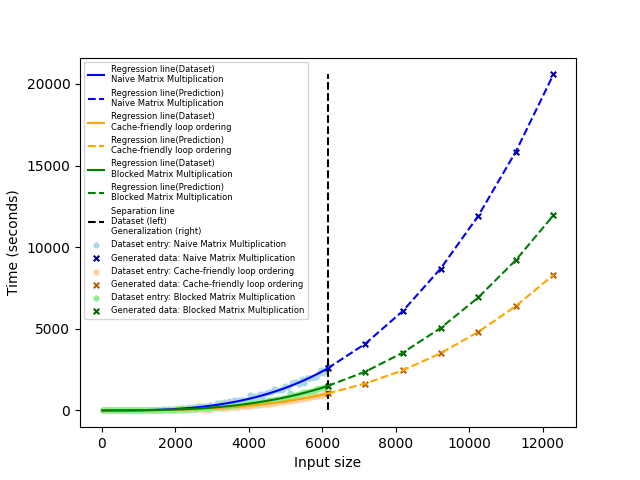
\includegraphics[width=0.8\textwidth]{mmn3023g}
\caption{Estimations based on the generalizations of the model tailored on the aquired dataset}
\end{figure}

\subsection{Strassen implementation}

For a while, we will leave the $O(n^3)$ matrix multiplication algorithms and focus on a new approach. As mentioned before, Strassen proposed a matrix multiplication algorithm with complexity $O(n^{log_{2}(7)}) \approx O(n^{2.80735})$. We aim at comparing this algorithm with the Cache-friendly loop ordering solution presented in the previous section.

In the traditional approach, without rComplexity analysis, we could not distinguish cases in which Strassen Algorithm could perform worse than any optimized $O(n^3)$ matrix multiplication solution.


\begin{fallacy}
Let $Alg1$ an algorithm with the complexity function $f_{1} \in \Theta(g_1(n))$  and $Alg2$ an algorithm with the complexity function $f_{2} \in \Theta(g_2(n))$. $Alg2$ must perform better than $Alg1$ \textit{for any size of input} in regard with the specified metric if $\lim_{n\to\infty} \dfrac{g_2(n)}{g_1(n)} = 0$.
\end{fallacy}


\begin{fallacy}
Adapted version for matrix multiplication:

Let $Alg1$ an algorithm with the complexity function $f_{1} \in \Theta(n^3)$  and $Alg2$ an algorithm with the complexity function $f_{2} \in \Theta(n^{2.80735})$. $Alg2$ must perform better than $Alg1$ \textit{for any size of input} in regard with the specified metric.
\end{fallacy}

Working with traditional complexity do not imply an universal increase in performance for $Alg2$, but an asymptotic comparison, while the fallacies presented in the previous statements assumed an universal behavior.

The correct manifest would be: $Alg2$ must perform better than $Alg1$ \textit{for sufficient large size of input} in regard with the specified metric if $\lim_{n\to\infty} \dfrac{g_2(n)}{g_1(n)} = 0$.

The collocation
\textit{"Sufficient large size of input"} is essential and it means that starting from a range of input size $n_{0}$ finite, better performances are obtained using $Alg2$.


\begin{figure}[H]
\centering
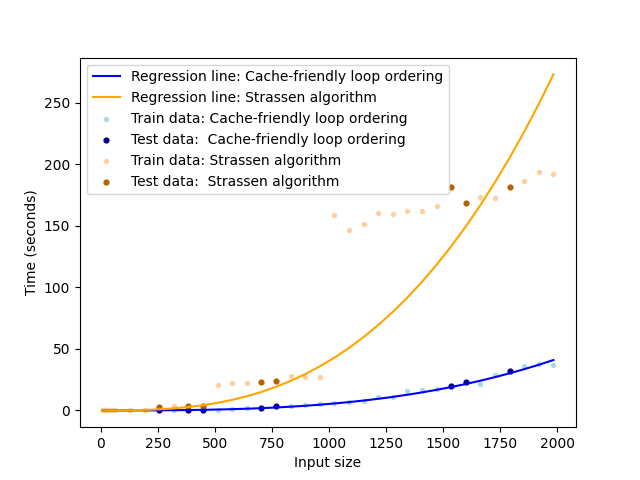
\includegraphics[width=0.8\textwidth]{mm328}
\caption{The regression line corresponding to the Cache-friendly loop ordering matrix multiplication algorithm is described by $f(n) = 5.23 \cdot 10^{-9} \cdot n^{3} $, while the regression line corresponding to the the Strassen algorithm is described by $g(n) = 1.59 \cdot 10^{-7} \cdot n^{2.80} $ . \\  Even if the asymptotic behavior for the Strassen algorithm is desired in comparison with the cubic performance, for finite input size the Cache-friendly loop ordering matrix multiplication algorithm can perform better, despite $\lim_{n\to\infty} \dfrac{g(n)}{f(n)} = 0$.  \\ The nature of the non-polynomial local behaviour of the Strassen algorithm is based on architecture considerations, such as the overhead introduced by specific function calls, stack manipulations and memory allocation and management computational cost. \\ \\ Results recorded on a x86\_64 Intel(R) Xeon(R) Gold 5218 CPU @ 2.30GHz with L1d cache: 32K, L1i cache: 32K, L2 cache: 1024K, L3 cache: 22528K, CPU max frequency: 3.9GHz.}
\end{figure}


\begin{pitfall}
Let $Alg1$ an algorithm with the complexity function $f_{1} \in \Theta(g_1(n))$  and $Alg2$ an algorithm with the complexity function $f_{2} \in \Theta(g_2(n))$ and $\lim_{n\to\infty} \dfrac{g_2(n)}{g_1(n)} = 0$.

Even if the $Alg1$ may perform better than $Alg2$ for some cases, the nature of this behavior is superficial and, in general, for regular routines, $Alg2$ will still perform better.
\end{pitfall}

\begin{pitfall}
Adapted version for matrix multiplication:

Even if the Cache-friendly loop ordering matrix multiplication algorithm may perform better than the Strassen algorithm for some cases, the nature of this behavior is superficial and, in general, for regular routines, the Strassen algorithm will still perform better.
\end{pitfall}

The key of the previous pitfalls is the meaning of \textit{"in general, for regular routines"}, because this phrase is extremely context-dependent. We will further calculate the separation point where the performances of Strassen algorithm catch up with (and overtake) the Cache-friendly loop ordering algorithm.

The point is provided by equalizing the two complexity functions:

$f(n) = 5.23 \cdot 10^{-9} \cdot n^{3} $ and $g(n) = 1.59 \cdot 10^{-7} \cdot n^{2.80} $

The nontrivial solution $n_{0}$ is obtained by solving $ 159 * n_{0}^{2.8} = 5.23* n_{0}^3 $, where $n_{0} \neq 0$. The solution is $n_{0} \approx 25970312 \approx 2.5 \cdot 10^7$.

\begin{figure}[H]
\centering
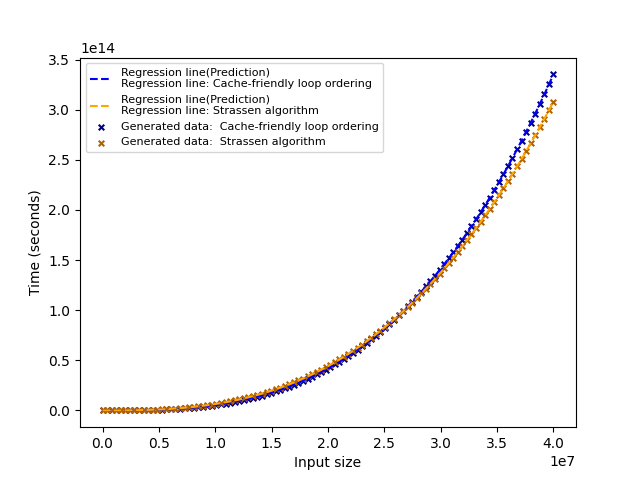
\includegraphics[width=0.8\textwidth]{mm328p}
\caption{Predictions for the Cache-friendly loop ordering matrix multiplication algorithm and Strassen algorithm based on acquired data. Remark the \textit{"catch up point"} between the two polynomial function for input size $\approx 2.5 \cdot 10^7$. }
\end{figure}

For any matrix multiplication task with input size greater than $\approx 2.5 \cdot 10^7$ (25 million element matrices), better results will be obtained using Strassen algorithm.

Remark that the total execution time (in seconds, on the tested computing machine) for 25 million element matrices, can be estimated to $g(2.5 \cdot 10^7) \approx f(2.5 \cdot 10^7) = 5.23 \cdot 10^{-9} \cdot (2.5 \cdot 10^7)^{3} \approx 8.13 \cdot 10^{13}$ seconds. This number $8.13 \cdot 10^{13} $ seconds is the equivalent of around 25 762 centuries.

If by "\textit{regular routines}" was meant multiplying \textit{25 million element matrices} and having the resources to await for 25 762 centuries for the result, than Strassen algorithm is the perfect solution for your problem \textit{(check also memory contraints, discussed in a short time)}. Otherwise, you should refer to a traditional approach.

\begin{figure}[H]
\makebox[\textwidth][c]{\parbox{1.2\textwidth}{%
\begin{subfigure}{.6\textwidth}
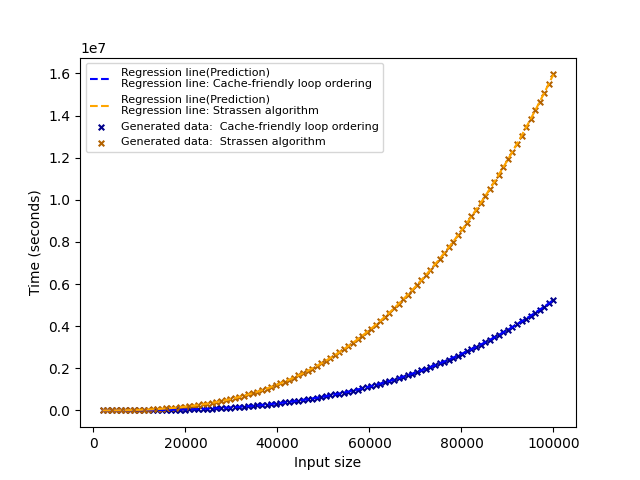
\includegraphics[width=\linewidth]{mm328p1.png}
\caption{Comparison between the two algorithms. \\Input size magnitude $\approx 10 ^ 6$}
\end{subfigure}%
\begin{subfigure}{.6\textwidth}
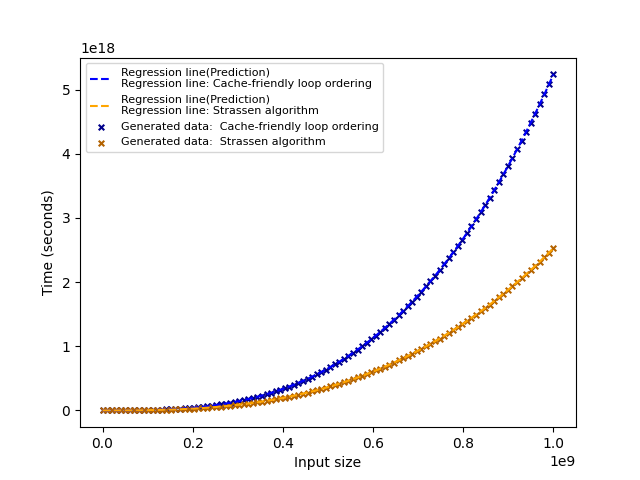
\includegraphics[width=\linewidth]{mm328p2.png}
\caption{Comparison between the two algorithms. \\Input size magnitude $\approx 10 ^ 9$}
\end{subfigure}

}}
\caption{Behaviour of Cache-friendly loop ordering matrix multiplication algorithm and Strassen algorithm based on predictions for different ranges of input.}
\end{figure}


\subsection{Memory considerations}

Up to this point, the only metric described in the prediction process of tailoring a complexity function was the \textbf{time} complexity. However, this is not the only resource that is important when designing algorithms and computer programs. A close match is represented by the total memory usage or peak memory usage of a computer program during the execution. Even if nowadays, memory is generally large enough to accommodate most of the possible algorithms, there are special situations in which memory management is critical.

The problem with the Strassen memory algorithm is that memory usage does not have a smooth improvement in growth. It varies in steps based on the powers of 2 (the cause is due to the recursion nature of the algorithm and at each iteration dividing in half).

Locally in intervals $[2^k, 2^{k+1} - 1]$, the memory increase in not huge, as the algorithm mentain a $n^2$ memory increase. However, generally the algorithm perform in a space complexity of $n^{log_{2}(7)}$.

\begin{figure}[H]
\makebox[\textwidth][c]{\parbox{1\textwidth}{%
\begin{subfigure}{.5\textwidth}
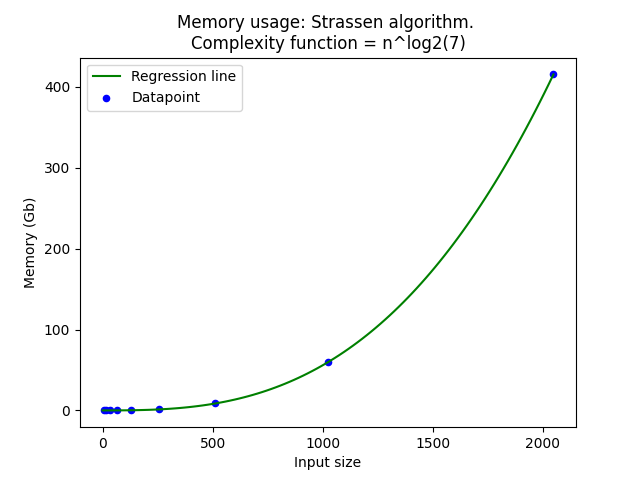
\includegraphics[width=\linewidth]{strassenusage2.png}
\caption{The total peak allocated memory usage \\ during the execution Strassen algorithm for \\  power-of-2 based input data}
\end{subfigure}%
\begin{subfigure}{.5\textwidth}
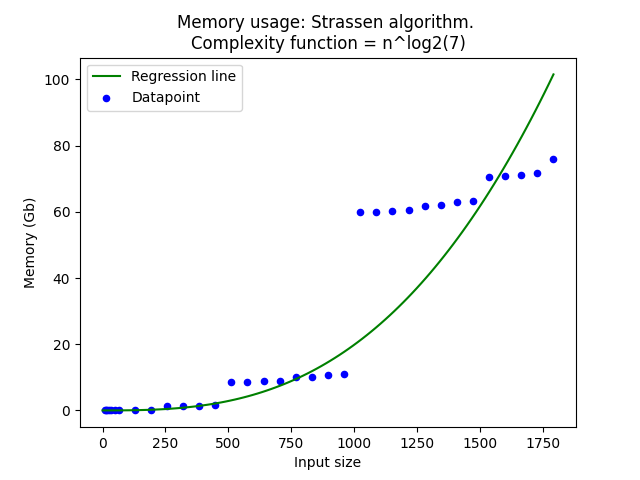
\includegraphics[width=\linewidth]{strassenusageall.png}
\caption{The total peak allocated memory usage \\ during the execution Strassen algorithm for\\  all recorded scenarios}
\end{subfigure}

}}
\caption{Peak memory usage - Strassen. Every double in input size produces a $7x$ increase in peak memory usage. Tailoring an complexity function of type $c \cdot n^{log_2(7)}$ provides a good evaluation. Using this appoximation, the maximum error at prediction is $7x$, while the average error is below $3x$. Power-of-2 based input data provides exact approximation.}
\end{figure}

\begin{pitfall}
Let $Alg1$ an algorithm with the complexity function $f_{1} \in \Theta(g_1(n))$  and $Alg2$ an algorithm with the complexity function $f_{2} \in \Theta(g_2(n))$ and $\lim_{n\to\infty} \dfrac{g_2(n)}{g_1(n)} = 0$.

Even if the $Alg1$ may perform better than $Alg2$ for some cases, for large input size, $Alg2$ will perform better and we shall thereby \textbf{always} use it.
\end{pitfall}

\begin{pitfall}
Adapted version for matrix multiplication:

For regular routines, the Strassen algorithm will perform better than any $O(n^3)$ naive matrix-multiplication algorithm for extremely large input size and we shall thereby use it.
\end{pitfall}

In theory, a smaller time-complexity always produce better asymptotically performances. The problems arise when we address other architectural aspects. Consider that an various algorithms uses memory usage differentiated. In order to perform precisely, a required condition is that the peak memory usage during the execution of the algorithm is at most equal with the total storage capacity of the physical RAM (ignore additional issues such as operating system memory overhead or translation concerns as well as pagination).


\begin{figure}[H]
\makebox[\textwidth][c]{\parbox{1\textwidth}{%
\begin{subfigure}{.5\textwidth}
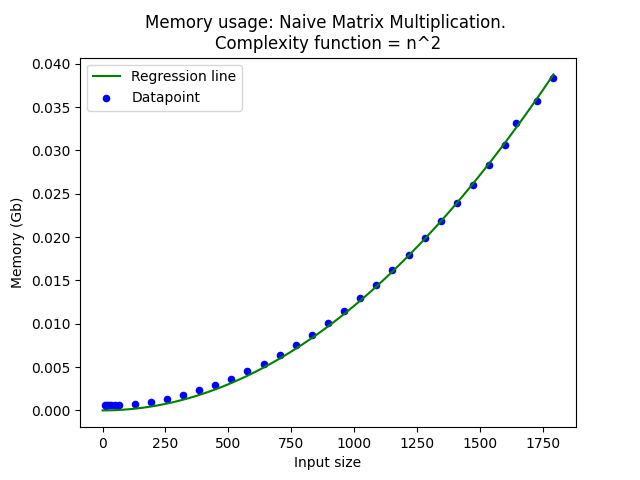
\includegraphics[width=\linewidth]{mn3.png}
\caption{The total peak allocated memory usage \\ during the execution of the Cache-friendly loop \\ ordering matrix multiplication algorithm}
\end{subfigure}%
\begin{subfigure}{.5\textwidth}
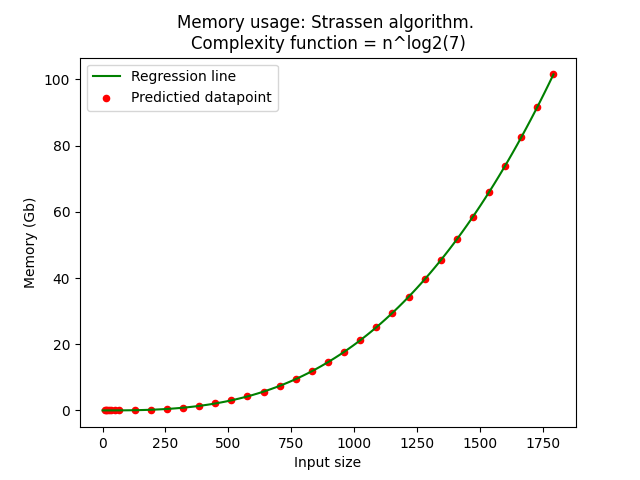
\includegraphics[width=\linewidth]{mstrassen.png}
\caption{The total peak allocated memory usage  \\ (estimated) for the execution of the \\ Strassen algorithm}
\end{subfigure}

}}
\caption{ Consider the peak memory usage for the last two algorithms analyzed. The behavior can be tailored by the individual associated memory complexity function: \\ $f_{cache\ friendly} = 1.20 \cdot 10^{-8} \cdot n^2 $ and  $f_{strassen} = 7.89 \cdot 10^{-8} \cdot n^{2.7} $ }
\end{figure}

Recall that the critical point in order to make Strassen algorithm perform better was estimated at around 25 million element matrices. For this value, the peak memory usage can be estimated at \textbf{7.43 ZB}. ($7.43 \cdot 10^{12}$ GB)
This amount of memory storage can be used to store \textbf{5 589 898} centuries of \textbf{1080p} digital video content \textit{(at a rate of 1.5GB/hour).} All this, in RAM memory.

Further extensions of this, using sophisticated group theory, are the Coppersmith–Winograd algorithm it is stressed nevertheless that such improvements are only of theoretical interest, since the huge constants involved in the complexity of fast matrix multiplication usually make these algorithms impractical. \cite{le2012faster}.

\begin{pitfall}
Never ever use Strassen algorithm.
\end{pitfall}
All the analyzed data was obtained by analyzing a specific implementation of the Strassen's Matrix Multiplication Algorithm. Not all algorithmic implementation performs the same. There may be optimizing techniques to overpass some issues, especially the deep recursion problems that raised. Also, there exists memory management tricks that substantially decrease the peak memory usage.

In fact, this algorithm is not \textbf{galactic} and is used in practice. A galactic algorithm has the property that it is faster than other algorithm for inputs that are sufficiently large, but where sufficiently large is enormous such that that the algorithm is never used in practice. \cite{le2012faster}.

All things summarized, the rComplexity metric provides powerful insights in comparison of different complexity algorithms and such example was observed in this chapter.


\section{Further reading}
The paper prepared additional resources for estimating rComplexity for algorithms with known Bachmann–Landau Complexity at the online codebase resource.
\begin{verbatim}
https://github.com/raresraf/rafMetrics/tree/master/rComplexity/samples
\end{verbatim}
This resource include analysis for the following algorithms:
\begin{itemize}
\item Naive Matrix Multiplication
\item Naive Matrix Multiplication (parallel)	
\item Naive Matrix Multiplication (OpenMP optimized)	
\item Cache-friendly loop ordering
\item Blocked Matrix Multiplication	
\item Strassen Matrix Multiplication	
\item NQueens (C)	
\item NQueens (python)	
\item Bubble Sort	
\item Insertion Sort	
\item Selection Sort	
\item Heap Sort	
\item Merge Sort	
\item Quick Sort	
\item SENPAI (serial): Simplified Evolutive N-body Processing and Analytics for Integration
\item SENPAI (parallel): Simplified Evolutive N-body Processing and Analytics for Integration
\item Chess Game
\item Web Crawler
\end{itemize}
